\addcontentsline{toc}{section}{Appendix} % Remove this if you don't want the appendix included in the table of contents.
\appendix

\section{MATLAB Code}\label{sec:matlab}

These MATLAB codes does not contain all the code from the project, but the necessary code to solve the different problems. Subsection~\ref{subsec:10_2_m} and ~\ref{subsec:10_3_m} build on the same theory and therefore subsection~\ref{subsec:10_2_m} contain some of the code needed in problem 10.3. The last subsection contain the code for the nonlinear constraint for problem 10.4.

\subsection{oppg10\_2.m}\label{subsec:10_2_m}
\lstinputlisting{code/oppg10_2.m}
\subsection{oppg10\_3.m}\label{subsec:10_3_m}
\lstinputlisting{code/oppg10_3.m}
\subsection{oppg10\_4.m}\label{subsec:10_4_m}
\lstinputlisting{code/oppg10_4.m}
\subsection{nonlconst.m}\label{subsec:nonlconst_m}
\lstinputlisting{code/nonlconst.m}

\section{Simulink Diagrams}\label{sec:simulink}
The two first Simulink diagrams are presented in sections~\ref{sec:10.2} and ~\ref{sec:10.3}. Hence, only the simulink diagrams for problem 10.4 is presented here.

\begin{figure}[H]
    \centering
    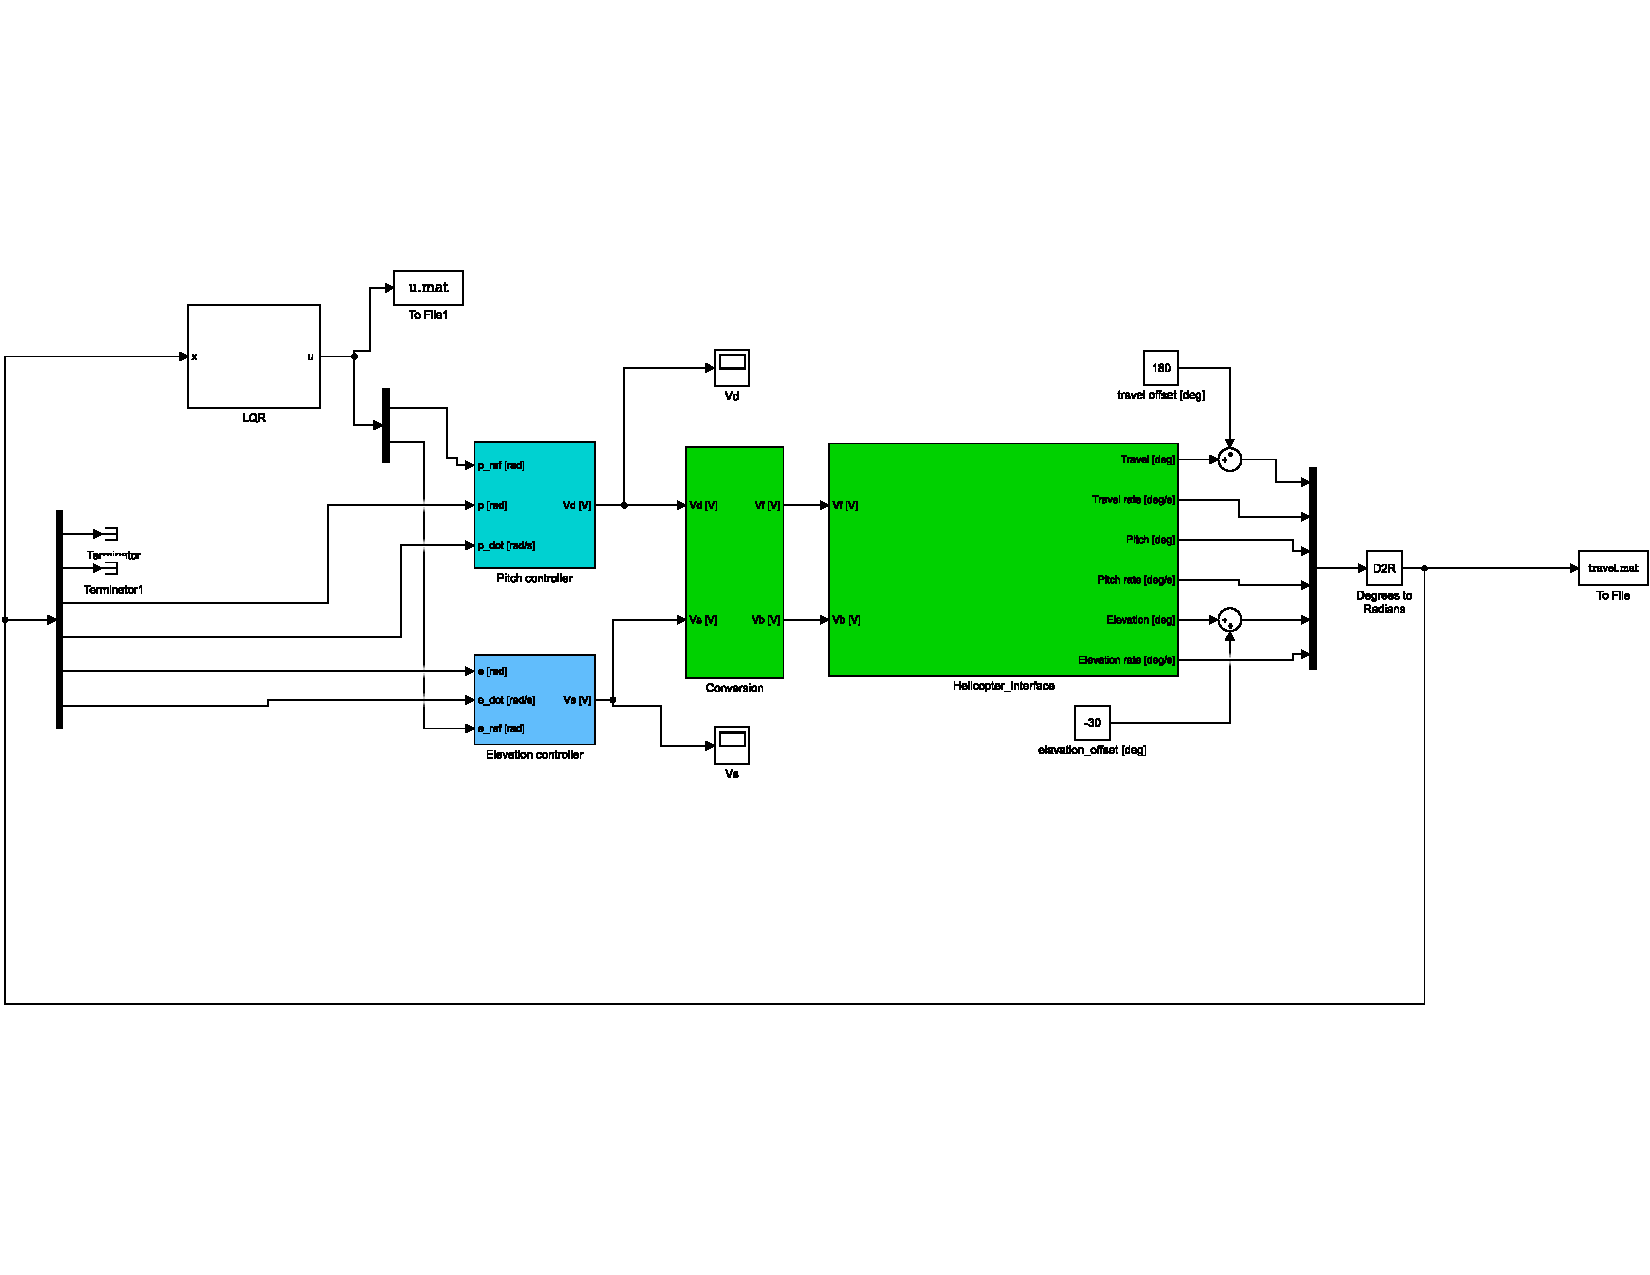
\includegraphics[scale=0.5]{data_10.4/simulink.pdf}
    \caption{Simulink model for problem 10.4}
    \label{fig:10_4_simulink}
\end{figure}
\begin{figure}[H]
    \centering
    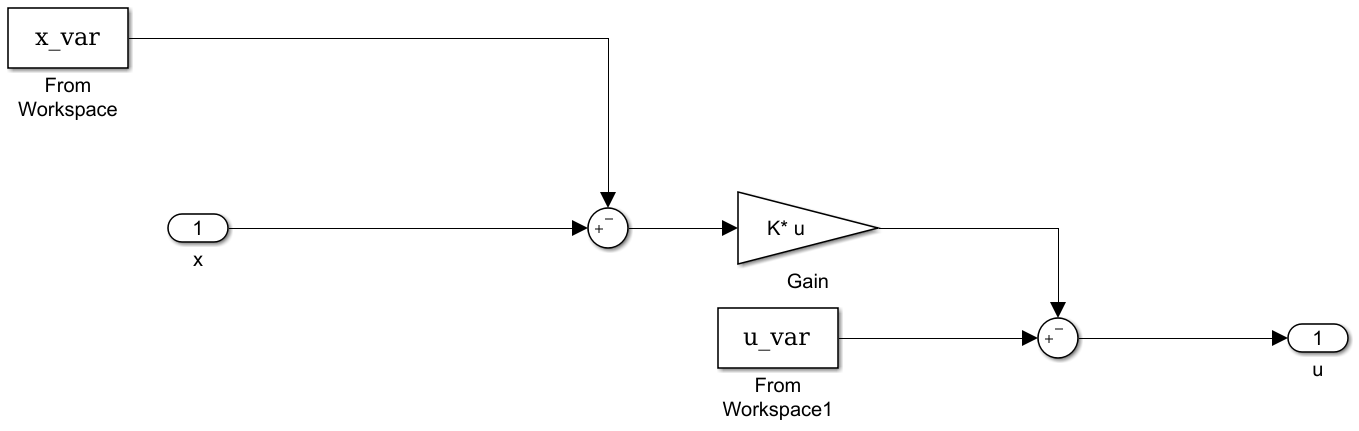
\includegraphics[width=1\linewidth]{data_10.4/simmodel_lqr.PNG}
    \caption{Simulink model showing the block diagram in LQR for problem 10.4}
    \label{fig:10_4_simulink_lqr}
\end{figure}
